\documentclass{article}
% [preprint] = name shown, "Preprint. Under review."; use [submission] for double-blind, [final] when accepted
\usepackage[preprint]{colm2026_conference}

\usepackage{amsmath,amssymb,amsthm}
\usepackage{booktabs}
\usepackage{graphicx}
\usepackage{hyperref}
\usepackage{url}
\usepackage{microtype}
\usepackage{xcolor}
\usepackage{lineno}
\usepackage{enumitem}
\usepackage{multirow}
\usepackage{pgfplots}
\pgfplotsset{compat=1.18}

\newtheorem{proposition}{Proposition}
\newcommand{\R}{\mathbb{R}}

\title{\textbf{TKV: Keep What the Basis Cannot Explain.\\
Frozen Low-Rank KV Caches and the Attention-Free,\\
Query-Agnostic Selection Criterion They Provide}}

\author{
  David Aror \\
  Independent Research \\
  \texttt{tejirid.aror@gmail.com}
}

\date{}

\begin{document}

\ifcolmsubmission
\linenumbers
\fi

\maketitle

\begin{abstract}
When a long context is compressed before the question is known --- cached
documents, multi-turn chat, prompt reuse --- a KV cache must decide which
tokens to keep without seeing the queries that will use them. Attention-based
selection (H2O, SnapKV) scores tokens by how \emph{past} queries attended to
them and requires materialized attention probabilities. We study \textbf{TKV}, a KV cache that fits a low-rank basis to pre-RoPE keys
during a short warmup and then freezes it, and show that its most useful
product is not the compressed storage but a \emph{signal}: each token's
projection residual $\lVert k - B^\top B k\rVert$ --- how much of the token the
basis cannot explain. We first show a limit on what any such rule can promise:
no query-agnostic policy that \emph{evicts} tokens can bound its error, because
a later query may align with exactly what was dropped. Keeping the
non-selected tokens as projections instead (\textbf{TKV-R}) admits a bound, and
ranking by the residual is what minimizes it --- making TKV-R the only
configuration in our comparison with a worst-case guarantee. It is also
competitive: at matched KV memory it ties the best query-agnostic method on
Mistral-7B (0.93 top-1 needle retrieval) and matches the best baseline on
TinyLlama-1.1B (0.77 vs.\ 0.77 H2O, ahead of 0.67 SnapKV and 0.60 StreamingLLM).
\textbf{TKV-S}, the evicting variant, uses the same residual without attention
scores or knowledge of the question. The bound holds because RoPE is a rotation; its evicting counterpart cannot
hold at all, which places TKV-S, H2O, SnapKV and KVzip alike in the heuristic
regime. It beats H2O on all three models tested (significantly on Mistral-7B and
Qwen2.5-14B), matches SnapKV on Mistral-7B, beats it on TinyLlama-1.1B (0.93
vs.\ 0.67), and trails it on Qwen2.5-14B (0.63 vs.\ 0.73, not significant).
A simple diagnostic --- where needle tokens fall in the residual distribution
--- predicts this ordering. Inside the cache the residual also beats attention-based selection at identical
memory and halves the perplexity cost of plain TKV on Mistral-7B. We report
where TKV as \emph{storage} does not pay off: at matched memory, eviction
remains better for perplexity. Along the way we correct
an invalid optimality claim for truncated Brand SVD updates and show that
frozen low-rank bases must be fit before RoPE.
\end{abstract}

%% ============================================================
\section{Introduction}
\label{sec:intro}

The key-value (KV) cache grows linearly with context and dominates inference
memory at long context. A large family of methods shrinks it by keeping only
some tokens \citep{streamingllm2023,h2o2023,snapkv2024,pyramidkv2024}. The
strongest of these select tokens by attention: H2O \citep{h2o2023} keeps tokens
that have received the most attention so far, and SnapKV \citep{snapkv2024}
keeps tokens attended by an observation window at the end of the prompt.
When the question is part of that window, SnapKV is close to lossless ---
it knows what will be asked. In many deployments it does not: a document is
cached before questions arrive, a conversation continues after compression,
or one prefix serves many requests. This \emph{query-agnostic} setting is
where selection is hardest \citep{kvzip2025}, and attention-based scores can
only extrapolate from queries that have already happened. They also require
attention probabilities, which fused kernels such as FlashAttention do not
expose.

TKV, the cache we started from, fits a rank-$R$ basis to the pre-RoPE keys of
a short warmup window and freezes it, storing every later token as
coefficients. Evaluated as \emph{storage}, that trade is not favorable
(Section~\ref{sec:prereq}); evaluated as a \emph{measurement}, the same basis
is valuable. For every later token it yields a residual: the part of the key
the basis cannot explain. A small basis captures what most
tokens share; a token that carries new information is one the basis explains
poorly. The residual is cheap --- an $r$-dimensional projection per token,
with $r{=}8$ in our main results --- and it is free in a low-rank KV cache,
which computes the projection anyway.

\textbf{Contributions.}
\begin{itemize}[leftmargin=*,itemsep=1pt]
  \item \textbf{Project, don't evict.} No query-agnostic rule that drops tokens
        can bound its error (Proposition~\ref{prop:noevict}); keeping them as
        projections can, and ranking by the residual minimizes that bound for
        every future query (Proposition~\ref{prop:cert}).
  \item \textbf{TKV-R}, the configuration that bound describes: at matched
        memory it ties the best query-agnostic method on Mistral-7B and the
        best baseline on TinyLlama-1.1B (Section~\ref{sec:main}).
  \item \textbf{TKV-S}, the evicting variant of the same criterion:
        attention-free, question-agnostic, $\mathcal{O}(rd)$ per token.
  \item \textbf{Matched-memory comparison} against StreamingLLM, H2O, SnapKV,
        random selection and query-aware SnapKV on TinyLlama-1.1B, Mistral-7B
        and Qwen2.5-14B, with significance tests (Section~\ref{sec:main}).
  \item \textbf{A predictor of when it works:} the residual percentile of the
        needed tokens tracks the method's standing across models
        (Section~\ref{sec:diag}).
  \item \textbf{Perplexity results} for the same criterion inside the TKV cache
        (Section~\ref{sec:tkvr}).
  \item \textbf{Corrections} to earlier claims about this line of work:
        truncated Brand updates are not globally optimal (we give a valid
        online certificate), frozen bases must be fit pre-RoPE, and a
        streaming Oja implementation pitfall (Sections~\ref{sec:prereq}
        and~\ref{sec:theory}).
\end{itemize}

%% ============================================================
\section{Setting}
\label{sec:setup}

\paragraph{Query-agnostic compression.}
A context of $T_c$ tokens is prefilled with exact attention and compressed
once; the question (positions $\ge T_c$) then attends to the compressed cache.
For each layer and KV head the cache keeps exactly $S{=}64$ sink tokens, the
last $W$ context tokens, and $M$ \emph{selected} middle tokens; other middle
tokens are evicted, or --- in a low-rank cache --- stored as rank-$R$
coefficients. Question tokens are always exact.

\paragraph{Selection criteria} (per layer and KV head, over middle tokens):
\emph{TKV-S residual} (ours, Section~\ref{sec:method}); \emph{SnapKV}: attention mass
from the last 32 context queries, max-pooled with kernel 7, summed over the
query heads sharing the KV head; \emph{H2O}: total attention mass received
from all context queries; \emph{random}. \emph{StreamingLLM} uses no selection
and spends the budget on a longer window. As a reference we also run
\emph{query-aware SnapKV}, whose observation window is the question itself.

\paragraph{Matched memory.}
Every configuration uses the same per-head KV storage relative to the full
cache: $(S + W + M)\,d$ entries for eviction; a rank-$R$ cache adds $Rd$ for the
basis and $R$ per \emph{compressed} token, so TKV-R with $M$ retained tokens
costs $(T - M)R + Rd + (S + W + M)\,d$ --- a token kept exactly does not also
store coefficients. At context 4096 and $d{=}128$ the budget is 0.594$\times$
(e.g.\ $W{=}256$, $M{=}2113$ for eviction; $W{=}2368$ for StreamingLLM); for
TinyLlama at context 2048, $d{=}64$, it is 0.672$\times$.

%% ============================================================
\section{TKV and Its Residual Criterion (TKV-S)}
\label{sec:method}

Let $B \in \R^{r\times d}$ have orthonormal rows spanning the top-$r$ right
singular vectors of the pre-RoPE keys of the first $T_0{=}512$ tokens. For a
middle token with pre-RoPE key $\mathbf{k}_j$, its residual is
\[
\rho_j = \lVert \mathbf{k}_j - B^\top B\,\mathbf{k}_j\rVert
       = \sqrt{\lVert\mathbf{k}_j\rVert^2 - \lVert B\mathbf{k}_j\rVert^2},
\]
and the rule keeps the $M$ middle tokens with the largest $\rho_j$. Scoring
costs $\mathcal{O}(rd)$ per token and uses no attention probabilities
(Table~\ref{tab:cost}); in a streaming cache it is a min-heap of capacity $M$
updated as tokens leave the window. Figure~\ref{fig:residual} (left) shows the
signal it exploits: needle tokens sit well above the median of the residual
distribution.

\paragraph{Why residuals.}
Let $\hat{\mathbf{k}}_j = B^\top B\mathbf{k}_j$ and let $\mathcal{R}_j$ be the
RoPE rotation at position $j$. For any query $\mathbf{q}$,
\begin{equation}
|\mathbf{q}^\top\mathcal{R}_j\mathbf{k}_j - \mathbf{q}^\top\mathcal{R}_j\hat{\mathbf{k}}_j|
\le \lVert\mathbf{q}\rVert\,\rho_j .
\label{eq:logit}
\end{equation}

\begin{proposition}[Query-agnostic certificate]
\label{prop:cert}
Suppose every non-retained middle token is represented by its projection
$\hat{\mathbf{k}}_j$, and let
$\varepsilon = \alpha\lVert\mathbf{q}\rVert\max_{j\ \text{not retained}}\rho_j$
for attention scale $\alpha$. Then the attention weights satisfy
$\lVert p - \hat p\rVert_1 \le e^{2\varepsilon} - 1$. Among all choices of $M$
retained tokens, keeping the $M$ largest residuals minimizes $\varepsilon$ for
every query simultaneously.
\end{proposition}

\emph{Proof sketch.} By \eqref{eq:logit} each scaled logit moves by at most
$\varepsilon$ (retained tokens by zero), so each softmax weight changes by a
factor in $[e^{-2\varepsilon}, e^{2\varepsilon}]$, giving the $\ell_1$ bound.
The bound depends on the retained set only through the largest remaining
residual, which the top-$M$ rule minimizes. \hfill$\square$

\paragraph{Why not simply take the best rank-$R$ basis?}
The Eckart--Young--Mirsky theorem gives the basis that minimizes
$\lVert K - \hat K\rVert_F$ --- the \emph{total} squared reconstruction error over
all tokens. The quantity that controls attention error is different: by
\eqref{eq:logit} and Proposition~\ref{prop:cert} the bound depends on
$\max_j \rho_j$ over the tokens that are \emph{not} kept exactly. A basis can be
Frobenius-optimal while leaving a single token badly represented, and that token
is precisely the one a later query may need. Averages and maxima pull in
different directions, which is why the useful decision here is not ``fit a better
basis'' but ``keep the tokens with the largest residual'': with a fixed rank, the
only remaining freedom is which residuals are allowed to remain.

Proposition~\ref{prop:cert} needs the non-selected tokens to be \emph{kept as
projections}, which is what TKV-R does (Section~\ref{sec:tkvr}); it says
nothing about evicting them outright. That is not an artifact of our analysis:
no query-agnostic rule can do better, as the next proposition shows.

\begin{proposition}[No query-agnostic guarantee under eviction]
\label{prop:noevict}
Fix any selection rule that drops a non-empty set $E$ of tokens without
representing them, chosen independently of the query. Suppose some
$j \in E$ is separable from the retained set $K$, i.e.\ there is a unit vector
$u$ with $u^\top k_j > \max_{l \in K} u^\top k_l$. Then, taking $\mathbf{q} = cu$
and letting $c \to \infty$, the attention output of the compressed cache
satisfies $\lVert o - \hat o\rVert \to \lVert \mathbf{v}_j - \mathbf{v}_{l^*}\rVert$,
where $l^*$ maximizes $u^\top k_l$ over $K$: the error is independent of how
many tokens were kept and of the criterion used to choose them.
\end{proposition}

\emph{Proof.} Dropping $E$ renormalizes the softmax over $K$, so with $m$ the
attention mass on $E$ we have $\lVert p - \hat p\rVert_1 = 2m$ and
$o - \hat o = \sum_{E} p_l \mathbf{v}_l - \frac{m}{1-m}\sum_{K} p_l \mathbf{v}_l$.
As $c\to\infty$ with $\mathbf{q} = cu$, $p_j \to 1$ within the full cache and the
retained mass concentrates on $l^*$, giving the stated limit. \hfill$\square$

So the error of any evicting scheme is governed by the attention mass of the
dropped tokens, which no query-independent score can bound: a token may be
perfectly explained by the basis (tiny $\rho_j$), yet be the one a later query
attends to most. H2O, SnapKV and KVzip are in the same position --- they
estimate that mass from past queries or from reconstruction, with no worst-case
control either. Two consequences shape this paper: TKV-R, which keeps
projections, is the member of the family that admits a guarantee at all
(Proposition~\ref{prop:cert}), and TKV-S must be judged empirically, as an
attention-free heuristic, against the other heuristics
(Section~\ref{sec:main}). The residual is a natural ranking there because it
measures what the rest of the cache cannot reproduce, but it carries no
promise about attention mass.

\begin{figure}[t]
\centering
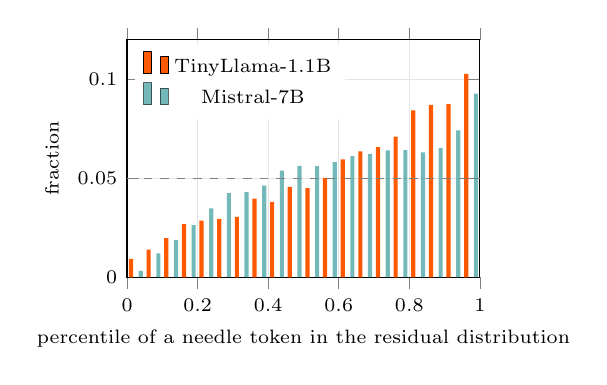
\begin{tikzpicture}
\begin{axis}[width=0.50\linewidth, height=4.6cm, ybar, bar width=1.5pt,
  xlabel={percentile of a needle token in the residual distribution},
  ylabel={fraction}, xmin=0, xmax=1, ymin=0, ymax=0.12,
  tick label style={font=\scriptsize}, label style={font=\scriptsize},
  legend style={font=\scriptsize, at={(0.02,0.98)}, anchor=north west, draw=none},
  ytick={0,0.05,0.1}, yticklabel style={/pgf/number format/fixed}, grid=major, grid style={gray!20}]
  \addplot[fill=orange!70!red, draw=none] coordinates {(0.025,0.0094) (0.075,0.0141) (0.125,0.0199)
    (0.175,0.0269) (0.225,0.0287) (0.275,0.0296) (0.325,0.0306) (0.375,0.0398) (0.425,0.0381)
    (0.475,0.0457) (0.525,0.0451) (0.575,0.0503) (0.625,0.0596) (0.675,0.0637) (0.725,0.0658)
    (0.775,0.0711) (0.825,0.0843) (0.875,0.0871) (0.925,0.0875) (0.975,0.1028)};
  \addlegendentry{TinyLlama-1.1B}
  \addplot[fill=teal, draw=none, opacity=0.55] coordinates {(0.025,0.0033) (0.075,0.0121) (0.125,0.0188)
    (0.175,0.0264) (0.225,0.0349) (0.275,0.0426) (0.325,0.0431) (0.375,0.0463) (0.425,0.0539)
    (0.475,0.0563) (0.525,0.0562) (0.575,0.0582) (0.625,0.0613) (0.675,0.0624) (0.725,0.0641)
    (0.775,0.0643) (0.825,0.0631) (0.875,0.0654) (0.925,0.0743) (0.975,0.0928)};
  \addlegendentry{Mistral-7B}
  \draw[dashed, gray] (axis cs:0,0.05) -- (axis cs:1,0.05);
\end{axis}
\end{tikzpicture}\hspace{-0.4cm}
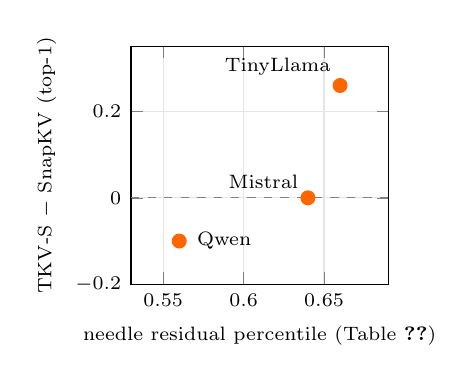
\begin{tikzpicture}
\begin{axis}[width=0.40\linewidth, height=4.6cm,
  xlabel={needle residual percentile (Table~\ref{tab:diag})},
  ylabel={TKV-S $-$ SnapKV (top-1)}, xmin=0.53, xmax=0.69, ymin=-0.2, ymax=0.35,
  tick label style={font=\scriptsize}, label style={font=\scriptsize},
  grid=major, grid style={gray!20}]
  \addplot[only marks, mark=*, mark size=2.5pt, color=orange!80!red]
    coordinates {(0.66,0.26) (0.64,0.0) (0.56,-0.10)};
  \node[font=\scriptsize, anchor=south east] at (axis cs:0.66,0.26) {TinyLlama};
  \node[font=\scriptsize, anchor=south east] at (axis cs:0.64,0.0) {Mistral};
  \node[font=\scriptsize, anchor=west] at (axis cs:0.565,-0.10) {Qwen};
  \draw[dashed, gray] (axis cs:0.53,0) -- (axis cs:0.69,0);
\end{axis}
\end{tikzpicture}
\caption{Left: where needle tokens fall in the residual distribution of middle
tokens (rank-8 basis; one entry per layer $\times$ KV head $\times$ needle token;
dashed line = no signal). Both models put needle tokens well above the median
(mean percentile 0.65 TinyLlama, 0.62 Mistral). Right: that separability
predicts how TKV-S compares with SnapKV (Section~\ref{sec:main}).}
\label{fig:residual}
\end{figure}

\begin{table}[t]
\centering
\caption{What each criterion needs, per token of context, to decide what to keep.}
\label{tab:cost}
\small
\setlength{\tabcolsep}{3pt}
\begin{tabular}{lllc}
\toprule
Criterion & Signal & Selection cost & Attn.\ probs? \\
\midrule
StreamingLLM & position only & $\mathcal{O}(1)$ & no \\
H2O & attention, all past queries & accumulate over $T$ queries & yes \\
SnapKV & attention, observation window & extra attention pass & yes \\
KVzip \citep{kvzip2025} & context reconstruction & extra forward pass(es) & no \\
\textbf{TKV-S (ours)} & pre-RoPE key projection & $\mathcal{O}(rd)$, $r{=}8$ & no \\
\bottomrule
\end{tabular}
\end{table}

\paragraph{A known weakness.} Tokens inside the warmup window helped fit $B$
and so have deflated residuals. A needle placed there (depth 0.1 in our 4K
prompts) is under-selected, increasingly so at larger $r$
(Section~\ref{sec:main}). Scoring each warmup half against a basis fit on the
other half (cross-fitting) recovered those needles on TinyLlama but lost
others, lowering overall accuracy at $r{=}8$ (0.93$\to$0.83); we do not use it.

%% ============================================================
\section{Experiments}
\label{sec:results}

\paragraph{Protocol.}
TinyLlama-1.1B (context 2048), Mistral-7B-v0.1 \citep{mistral2023} and
Qwen2.5-14B \citep{qwen25} (context 4096), bfloat16. A one-sentence needle
(``The special code word is \emph{blue}.'') is inserted into WikiText-2 text
\citep{merity2017} at depths 0.1/0.3/0.5/0.7/0.9 with six different needle
words per depth (30 prompts per configuration); the prompt ends with a
question whose answer is the needle word \citep{niah2023}. We report top-1
accuracy of the answer token and its mean probability. Compression is
simulated in one teacher-forced pass with a custom attention function; with a
window covering the context, or a full-rank basis, it reproduces exact
logits (relative error $<10^{-6}$). Significance is two-sided Fisher's exact
test on correct/incorrect counts.

\subsection{Query-agnostic selection}
\label{sec:main}

\begin{table}[t]
\centering
\caption{Query-agnostic needle retrieval at matched KV memory: top-1 accuracy
(mean $P$ of the answer). TKV-S ($r$) evicts non-selected tokens and uses a
rank-$r$ scoring basis; TKV-R keeps them as rank-$R$ projections and is the only
configuration with a worst-case guarantee (Proposition~\ref{prop:cert}):
$R{=}16$, $W{=}256$ (TinyLlama), $R{=}32$, $W{=}512$ (Mistral) and $R{=}8$,
$W{=}256$ (Qwen), each chosen as the best of three allocations on a disjoint
set of 30 dev prompts (haystack windows shifted by 20 contexts).
Query-aware SnapKV sees the question and is a reference, not a competitor.}
\label{tab:main}
\small
\begin{tabular}{lccc}
\toprule
& TinyLlama-1.1B & Mistral-7B & Qwen2.5-14B \\
& (0.672$\times$) & (0.594$\times$) & (0.594$\times$) \\
\midrule
Exact (full cache)       & 1.00 (0.83) & 1.00 (0.74) & 1.00 (0.83) \\
\midrule
StreamingLLM             & 0.60 (0.53) & 0.60 (0.45) & 0.60 (0.51) \\
H2O                      & 0.77 (0.60) & 0.67 (0.36) & 0.33 (0.38) \\
SnapKV (query-agnostic)  & 0.67 (0.55) & \textbf{0.93} (0.55) & \textbf{0.73} (0.62) \\
Random                   & 0.37 (0.33) & 0.77 (0.32) & -- \\
\textbf{TKV-S ($r{=}8$)} & \textbf{0.93} (0.75) & \textbf{0.93} (0.55) & 0.63 (0.58) \\
\textbf{TKV-R} (projection, guaranteed) & 0.77 (0.57) & \textbf{0.93} (0.53) & 0.53 (0.44) \\
TKV-S ($r{=}16$)         & -- & 0.80 (0.56) & -- \\
TKV-S ($r{=}32$)         & 0.73 (0.61) & 0.80 (0.58) & -- \\
\midrule
\emph{SnapKV (query-aware)} & \emph{1.00 (0.83)} & \emph{1.00 (0.74)} & -- \\
\bottomrule
\end{tabular}
\end{table}

\begin{table}[t]
\centering
\caption{TKV-S ($r{=}8$) vs.\ each baseline: correct answers out of 30 and
Fisher's exact $p$.}
\label{tab:sig}
\small
\begin{tabular}{lccc}
\toprule
TKV-S vs. & TinyLlama-1.1B & Mistral-7B & Qwen2.5-14B \\
\midrule
StreamingLLM & 28 vs 18, $p{=}0.005$ & 28 vs 18, $p{=}0.005$ & 19 vs 18, $p{=}1.0$ \\
H2O          & 28 vs 23, $p{=}0.15$  & 28 vs 20, $p{=}0.021$ & 19 vs 10, $p{=}0.038$ \\
SnapKV       & 28 vs 20, $p{=}0.021$ & 28 vs 28, $p{=}1.0$   & 19 vs 22, $p{=}0.58$ \\
\bottomrule
\end{tabular}
\end{table}

Table~\ref{tab:main} shows that without seeing the question, TKV-S at
$r{=}8$ is the best or tied-best query-agnostic method on
TinyLlama and Mistral-7B and second on Qwen2.5-14B. It beats H2O on all three
models (significantly on the two larger ones, Table~\ref{tab:sig}); H2O's
cumulative attention favors early tokens and collapses at late depths on the
larger models (mean $P$ at depth 0.9: 0.07 on Mistral, 0.03 on Qwen). It
matches SnapKV on Mistral-7B, beats it on TinyLlama, and trails it on
Qwen2.5-14B by a non-significant margin. Evicting the same number of tokens at
random is surprisingly competitive on Mistral (0.77), which is a reminder that
at 0.59$\times$ memory more than half of the middle tokens survive; TKV-S
still improves on it (28 vs 23, $p{=}0.15$). Larger scoring bases
lose the depth-0.1 needle that lies inside the warmup window (mean $P$ 0.00 at
$r{=}32$ on Mistral) while doing well elsewhere, the weakness described in
Section~\ref{sec:method}. Query-aware SnapKV remains near-exact, so the query-agnostic setting leaves
real headroom.

\paragraph{The guaranteed variant is also competitive.} TKV-R keeps the
non-selected tokens as projections, so Proposition~\ref{prop:cert} applies and
Proposition~\ref{prop:noevict} does not: it is the only configuration in the
comparison with a worst-case bound. Under the storage accounting of
Section~\ref{sec:setup} --- a retained token does not also pay for coefficients
it no longer needs --- TKV-R matches the best query-agnostic method on
Mistral-7B (0.93, tied with TKV-S and SnapKV), ties H2O on TinyLlama (0.77,
ahead of SnapKV at 0.67 and StreamingLLM at 0.60), and reaches 0.53 on
Qwen2.5-14B, ahead of H2O (0.33) but behind SnapKV, as its low residual
separability predicts (Section~\ref{sec:diag}). Its rank/window split is
chosen on a disjoint dev set: that choice reproduces the reported allocation on
Mistral-7B and Qwen2.5-14B, and on TinyLlama selects $R{=}16$ (test 0.77)
rather than the $R{=}8$ that would have been best in hindsight (0.80). How the budget is
split matters: the same memory spent as rank 32 with a 512-token window is
worth 0.93 on Mistral but 0.27 on Qwen, where rank 8 with a 256-token window
gives 0.53. Scoring by the
full two-term bound of Proposition~\ref{prop:cert} rather than by $\rho^k$
alone selects the same tokens (0.77 vs.\ 0.77 on Mistral at $R{=}8$), because
the bound is monotone in $\max\rho^k$ and its value-residual term is second
order; ranking by the key residual is therefore bound-optimal, not an
approximation of it.

\subsection{When does TKV-S work?}
\label{sec:diag}

\begin{table}[t]
\centering
\caption{Residual separability of needle tokens and the method's standing.
Needle tokens kept: fraction of needle-sentence tokens kept exact for the
final query under random vs.\ residual selection inside a low-rank cache
(averaged over layers, heads and prompts); percentile: mean position of needle
tokens in the residual distribution (0.5 = indistinguishable).}
\label{tab:diag}
\small
\begin{tabular}{lcccc}
\toprule
& \multicolumn{2}{c}{Needle tokens kept} & TKV residual & TKV-S vs.\ SnapKV \\
Model & random & TKV-S & percentile & (query-agnostic) \\
\midrule
TinyLlama-1.1B & 0.144 & 0.244 (1.7$\times$) & 0.66 & better \\
Mistral-7B     & 0.262 & 0.381 (1.5$\times$) & 0.64 & tied \\
Qwen2.5-14B    & 0.260 & 0.291 (1.1$\times$) & 0.56 & worse \\
\bottomrule
\end{tabular}
\end{table}

The criterion can only help if the tokens a later query needs stand out in
residual. Figure~\ref{fig:residual} shows the distribution directly, and
Table~\ref{tab:diag} measures its effect: on TinyLlama and Mistral,
needle tokens sit at the 64th--66th residual percentile and are kept
1.5--1.7$\times$ more often than chance; on Qwen2.5-14B they sit at the 56th
percentile. The ordering matches TKV-S's standing against SnapKV exactly. Removing a possible key-bias effect by mean-centering the basis did
not change Qwen's separability (0.291 kept with and without centering).
Separability can be measured on a calibration prompt before deployment.

\subsection{Residual selection inside the TKV cache (TKV-R)}
\label{sec:tkvr}

TKV freezes a rank-$R$ pre-RoPE basis after the warmup and stores every later
token as coefficients; there the residual is free and
Proposition~\ref{prop:cert} applies exactly --- this is the only setting in
the family with a worst-case guarantee, by Proposition~\ref{prop:noevict}. TKV-R keeps the top-$M$
residual tokens exact on top of the coefficients. At identical $R$, $W$, $M$
in the query-agnostic setting (TinyLlama, $R{=}8$, $W{=}768$, $M{=}280$),
choosing the exact tokens by residual reaches 0.67 needle accuracy, against
0.43 by SnapKV scores and 0.40 by H2O scores: inside a low-rank cache,
attention-based selection is clearly worse, while the residual is the right
signal.

\begin{table}[t]
\centering
\caption{TKV-R in a streaming low-rank cache at matched memory (0.594$\times$,
context 4096): WikiText-2 perplexity on 30 windows (increase over exact) and
needle top-1 accuracy (15 prompts; the cache is compressed as tokens stream,
including the question). Unlike Table~\ref{tab:main}, this streaming accounting
charges every middle token for its coefficients even when it is also kept
exact, so the TKV-R rows spend slightly less than the budget.
Exact: Mistral 4.595, Qwen 3.977. $R$/$W$/$f$: rank,
window, fraction of middle tokens kept exact.}
\label{tab:tkvr}
\small
\begin{tabular}{lccccc}
\toprule
& & \multicolumn{2}{c}{Mistral-7B} & \multicolumn{2}{c}{Qwen2.5-14B} \\
\cmidrule(lr){3-4}\cmidrule(lr){5-6}
Method & $R$ / $W$ / $f$ & PPL & Needle & PPL & Needle \\
\midrule
StreamingLLM            & -- / 2368 / --  & \textbf{+1.0\%} & 0.60 & \textbf{+1.0\%} & \textbf{0.60} \\
TKV (storage only)      & 64 / 256 / --   & +5.6\% & 0.87 & +5.3\% & 0.20 \\
OjaKV (corrected)       & 64 / 256 / --   & +5.2\% & \textbf{0.93} & +5.1\% & -- \\
TKV, larger window      & 16 / 1840 / --  & +1.9\% & 0.40 & +1.7\% & 0.33 \\
TKV + random retention  & 16 / 768 / 0.33 & +3.7\% & 0.20 & +2.8\% & 0.20 \\
\textbf{TKV-R}          & 16 / 768 / 0.33 & +1.8\% & 0.73 & +1.3\% & 0.20 \\
\textbf{TKV-R}          & 32 / 512 / 0.23 & +2.5\% & \textbf{0.93} & +1.9\% & 0.20 \\
\bottomrule
\end{tabular}
\end{table}

Table~\ref{tab:tkvr} shows the perplexity side. On Mistral-7B, TKV-R at
rank 32 matches the best low-rank retrieval (0.93) at less than half the
perplexity cost of plain TKV or OjaKV ($+2.5\%$ vs.\ $+5.6\%$/$+5.2\%$), and at
rank 16 it equals the perplexity of spending the same memory on a longer
window ($+1.8\%$ vs.\ $+1.9\%$) while nearly doubling retrieval (0.73 vs.\
0.40). Random retention is worse on both axes on Mistral. On Qwen2.5-14B TKV-R brings
perplexity close to eviction but does not improve retrieval, consistent with
Table~\ref{tab:diag}. Eviction alone remains best for perplexity on both
models. The simulated retention set (top $\lfloor f\,n_i\rfloor$ residuals of
query $i$'s $n_i$ middle tokens) is a subset of what a fixed-capacity heap
keeps and equals it for the final query, so these numbers are conservative
for perplexity and exact for final-position retrieval.

\subsection{Where TKV as storage does not pay off, and what it needs}
\label{sec:prereq}

\paragraph{Pre-RoPE bases.} RoPE rotates keys by position, so a basis frozen
on early post-RoPE keys cannot span later ones. At rank 64 a post-RoPE basis
costs $+11.5\%$ / $+10.1\%$ perplexity (Mistral / Qwen) against $+5.6\%$ /
$+5.3\%$ pre-RoPE; on TinyLlama the post-RoPE variant is catastrophic
(perplexity 76.3 vs.\ 6.94 at rank 48). All results above use pre-RoPE keys.

\paragraph{Oja baselines.} A natural streaming Oja implementation --- including
our own first one --- stores each token's coefficients in the basis current at
its arrival but reconstructs with the final basis, and uses a step that is not
normalized by $\lVert\mathbf{x}\rVert^2$; this produced relative reconstruction
errors above 1.0 on real keys. We do not know whether the original OjaKV code
\citep{ojakov2025} shares the issue. Corrected and given the same warmup,
OjaKV is within 0.5\% of TKV's perplexity, including on a benchmark that
switches from prose to code after the warmup.

\paragraph{TKV as storage vs.\ eviction.} Without residual retention, eviction
beats the TKV cache at every budget (e.g.\ at 0.21$\times$ memory
$+9.5\%$ vs.\ $+19.8\%$ on Mistral, $+7.4\%$ vs.\ $+23.0\%$ on Qwen) and on
PG-19 \citep{rae2020}; a PyramidKV-style \citep{pyramidkv2024} rank schedule
was worse than uniform rank.

\paragraph{Decode cost.} On an NVIDIA L40S, one decode step for one layer
(8 KV $\times$ 4 query heads, $d{=}128$) over a frozen rank-32 basis costs
0.36\,ms at 32K tokens and 2.14\,ms at 128K, vs.\ 2.83 / 12.35\,ms for the full
cache and 1.31 / 3.33\,ms for OjaKV; at rank 64, 5.75\,ms at 128K. Residual
scoring for eviction adds one rank-8 projection per token.

%% ============================================================
\section{Correcting the Streaming-Warmup Guarantee}
\label{sec:theory}

Earlier versions of this work claimed that each truncated Brand update
\citep{brand2006} keeps the Eckart--Young--Mirsky (EYM) optimal rank-$R$
approximation of the whole token history. That is false: after truncation
the discarded directions are gone, so the next update factors
$A_t = \begin{bmatrix}\hat K_{t-1}\\ \mathbf{k}_t^\top\end{bmatrix}$, not
$K_t = \begin{bmatrix}K_{t-1}\\ \mathbf{k}_t^\top\end{bmatrix}$.

\begin{proposition}[What truncated Brand updates guarantee]
\label{prop:brand}
Let $\hat K_t$ be the best rank-$R$ approximation of $A_t$ and
$E_t = K_t - \hat K_t$. Then (i) $\hat K_t$ is EYM-optimal for $A_t$, the
previous truncated state augmented with the new token; and (ii)
$\lVert E_t\rVert_F \le \lVert E_{t_c}\rVert_F + \sum_{s=t_c+1}^{t}\sigma_{R+1}(A_s)$
after a cold start at $t_c$.
\end{proposition}

\emph{Proof.} (i) is Brand's construction plus EYM on $A_t$. For (ii),
$E_t = \begin{bmatrix}E_{t-1}\\ \mathbf{0}^\top\end{bmatrix} + (A_t - \hat K_t)$; since
$\mathrm{rank}(A_t)\le R{+}1$, exactly one singular value is discarded, so
$\lVert A_t - \hat K_t\rVert_F = \sigma_{R+1}(A_t)$, and the triangle
inequality gives the recursion. \hfill$\square$

Each $\sigma_{R+1}(A_t)$ is produced by the update, so a streaming warmup can
report a running certificate of its own error. The earlier per-token global
optimality corollaries are withdrawn. Our experiments fit the warmup basis by
exact SVD, which is optimal for the warmup window.

%% ============================================================
\section{Related Work}
\label{sec:related}

\textbf{Token selection.} StreamingLLM \citep{streamingllm2023} keeps sinks and
a recent window; H2O \citep{h2o2023}, Scissorhands \citep{scissorhands2023},
SnapKV \citep{snapkv2024} and PyramidKV \citep{pyramidkv2024} use attention
statistics. KVzip \citep{kvzip2025} targets the query-agnostic setting
directly, scoring KV pairs by how much the model needs them to reconstruct the
context; it is strong but requires additional forward passes, whereas the
residual criterion costs one small projection per token. We did not compare
against KVzip. \textbf{Low-rank and residual caches.} Palu \citep{palu2024},
LoRC \citep{lorc2024}, xKV \citep{xkv2025}, SVDq \citep{svdq2025}, STAR-KV
\citep{starkv2026} and PuzzleKV \citep{puzzlekv2026} factorize caches or
projections, and ShadowKV \citep{shadowkv2024} keeps a low-rank pre-RoPE key
cache; OjaKV \citep{ojakov2025} adapts the basis online. AnchorKV
\citep{anchorkv2026} keeps anchor tokens exact and refines the tokens whose
approximation most affects the output, and DeltaKV \citep{deltakv2026} stores
residuals against retrieved reference tokens. Our criterion shares the goal of
spending exact storage where an approximation is worst, but uses the residual
of a single small online basis, requires no attention or output signal, and
applies both to pure eviction and to low-rank caches.

%% ============================================================
\section{Limitations}
\label{sec:limitations}

The evidence is a single synthetic needle format at 2K--4K tokens with 30
prompts per cell; RULER, LongBench and multi-needle or multi-hop tasks, and
contexts of 32K and beyond, are needed before claiming general retrieval
gains. Results are model-dependent (weaker than SnapKV on Qwen2.5-14B), and
the scoring rank and warmup placement matter. TKV-S is a heuristic: by
Proposition~\ref{prop:noevict} no query-agnostic evicting rule admits a
worst-case guarantee, so its standing rests on the empirical comparison alone.
TKV-R's rank/window split is chosen on a disjoint dev set of 30 prompts, so its
reported numbers are not tuned on the test prompts; the baselines have no
comparable hyperparameter and were run at fixed settings. We compare against H2O and
SnapKV as described in Section~\ref{sec:setup} but not KVzip or quantization.
Compression is simulated in a teacher-forced pass with memory accounted
analytically, and residual eviction was not timed end to end.

%% ============================================================
\section{Conclusion}

TKV's frozen pre-RoPE basis earns its keep less as storage than as a
measurement: the residual it produces is a cheap, attention-free,
query-agnostic signal of which tokens a KV cache should keep. Because no
evicting rule can promise anything to a query it has not seen, the variant that
keeps projections (TKV-R) is the one with a guarantee --- and at matched memory
it ties the best query-agnostic method on Mistral-7B and the best baseline
on TinyLlama.
At matched memory TKV-S consistently beats H2O, matches or beats SnapKV on two
of three models without seeing the question, and --- inside the TKV cache
(TKV-R) --- beats attention-based selection outright, halving TKV's perplexity
cost at equal retrieval. A one-number diagnostic predicts
where it helps. On the theory side we withdraw an incorrect optimality claim for truncated
Brand updates in favor of a valid online certificate, and we show that keeping
projections --- not evicting --- is what makes a query-agnostic guarantee
possible at all.

%% ============================================================
\small
\bibliography{colm2026_conference}
\bibliographystyle{colm2026_conference}

\appendix
\section{Additional Numbers}
\label{app:numbers}

\textbf{Needle probability by depth, query-agnostic (mean $P$ at depths
0.1/0.3/0.5/0.7/0.9).} Mistral-7B: exact 0.70/0.74/0.74/0.72/0.78;
StreamingLLM 0.00/0.00/0.74/0.73/0.79; H2O 0.60/0.49/0.39/0.24/0.07; SnapKV
0.41/0.50/0.42/0.63/0.77; random 0.32/0.26/0.29/0.40/0.33; residual $r{=}8$
0.23/0.53/0.62/0.65/0.70; residual $r{=}32$ 0.00/0.72/0.67/0.72/0.79; TKV-R
(low-rank, $R{=}32$, $W{=}512$, $M{=}1068$) 0.23/0.56/0.52/0.60/0.75, accuracy
0.93. Qwen2.5-14B: exact 0.86/0.82/0.87/0.81/0.76; StreamingLLM
0.00/0.00/0.86/0.87/0.82; H2O 0.80/0.62/0.22/0.22/0.03; SnapKV
0.40/0.46/0.71/0.78/0.76; residual $r{=}8$ 0.11/0.72/0.68/0.77/0.60.
TinyLlama: residual $r{=}8$ 0.52/0.74/0.84/0.82/0.84; H2O
0.55/0.70/0.60/0.37/0.81; SnapKV 0.52/0.42/0.29/0.69/0.82.

\textbf{Cross-fitted residuals (TinyLlama).} $r{=}8$: accuracy 0.83, mean $P$
0.71 (vs.\ 0.93, 0.75 without); $r{=}32$: 0.77, 0.62 (vs.\ 0.73, 0.61).

\textbf{Rank vs.\ window without retention (0.594$\times$, streaming).}
$R$ = 0/16/32/48/64 with $W$ = 2368/1840/1312/784/256: Mistral perplexity
4.640/4.682/4.712/4.763/4.853, needle accuracy 0.60/0.40/0.53/0.60/0.87; Qwen
4.018/4.046/4.080/4.117/4.189 and 0.60/0.33/0.33/0.27/0.20.

\end{document}
